\documentclass{article}
\usepackage[utf8]{inputenc}
\usepackage{geometry}
\usepackage{graphicx}
\usepackage{float}
\usepackage{listings}
\usepackage{xcolor}
\usepackage{tcolorbox}
\geometry{margin=1in}

\lstset{
    basicstyle=\ttfamily\small,
    breaklines=true,
    frame=single,
    backgroundcolor=\color{gray!10},
    columns=flexible
}

\lstdefinestyle{bash}{
    language=bash,
    keywordstyle=\color{blue}\bfseries,
    commentstyle=\color{green!60!black}
}

% Define document metadata in the preamble
\title{\bfseries Debugging pods in a Kubernetes cluster}
\author{Souvik Sarkar \\ \texttt{sounix000@gmail.com}} % Applied your signature author block
\date{February 6, 2023}

\begin{document}

\maketitle % Generates your standard title, author, and email block

\section*{Overview}

Pods are the smallest deployable units in Kubernetes and critical to application functionality. Debugging pods helps ensure applications run smoothly, scale seamlessly, and use cluster resources effectively.

\begin{figure}[H]
    \centering
    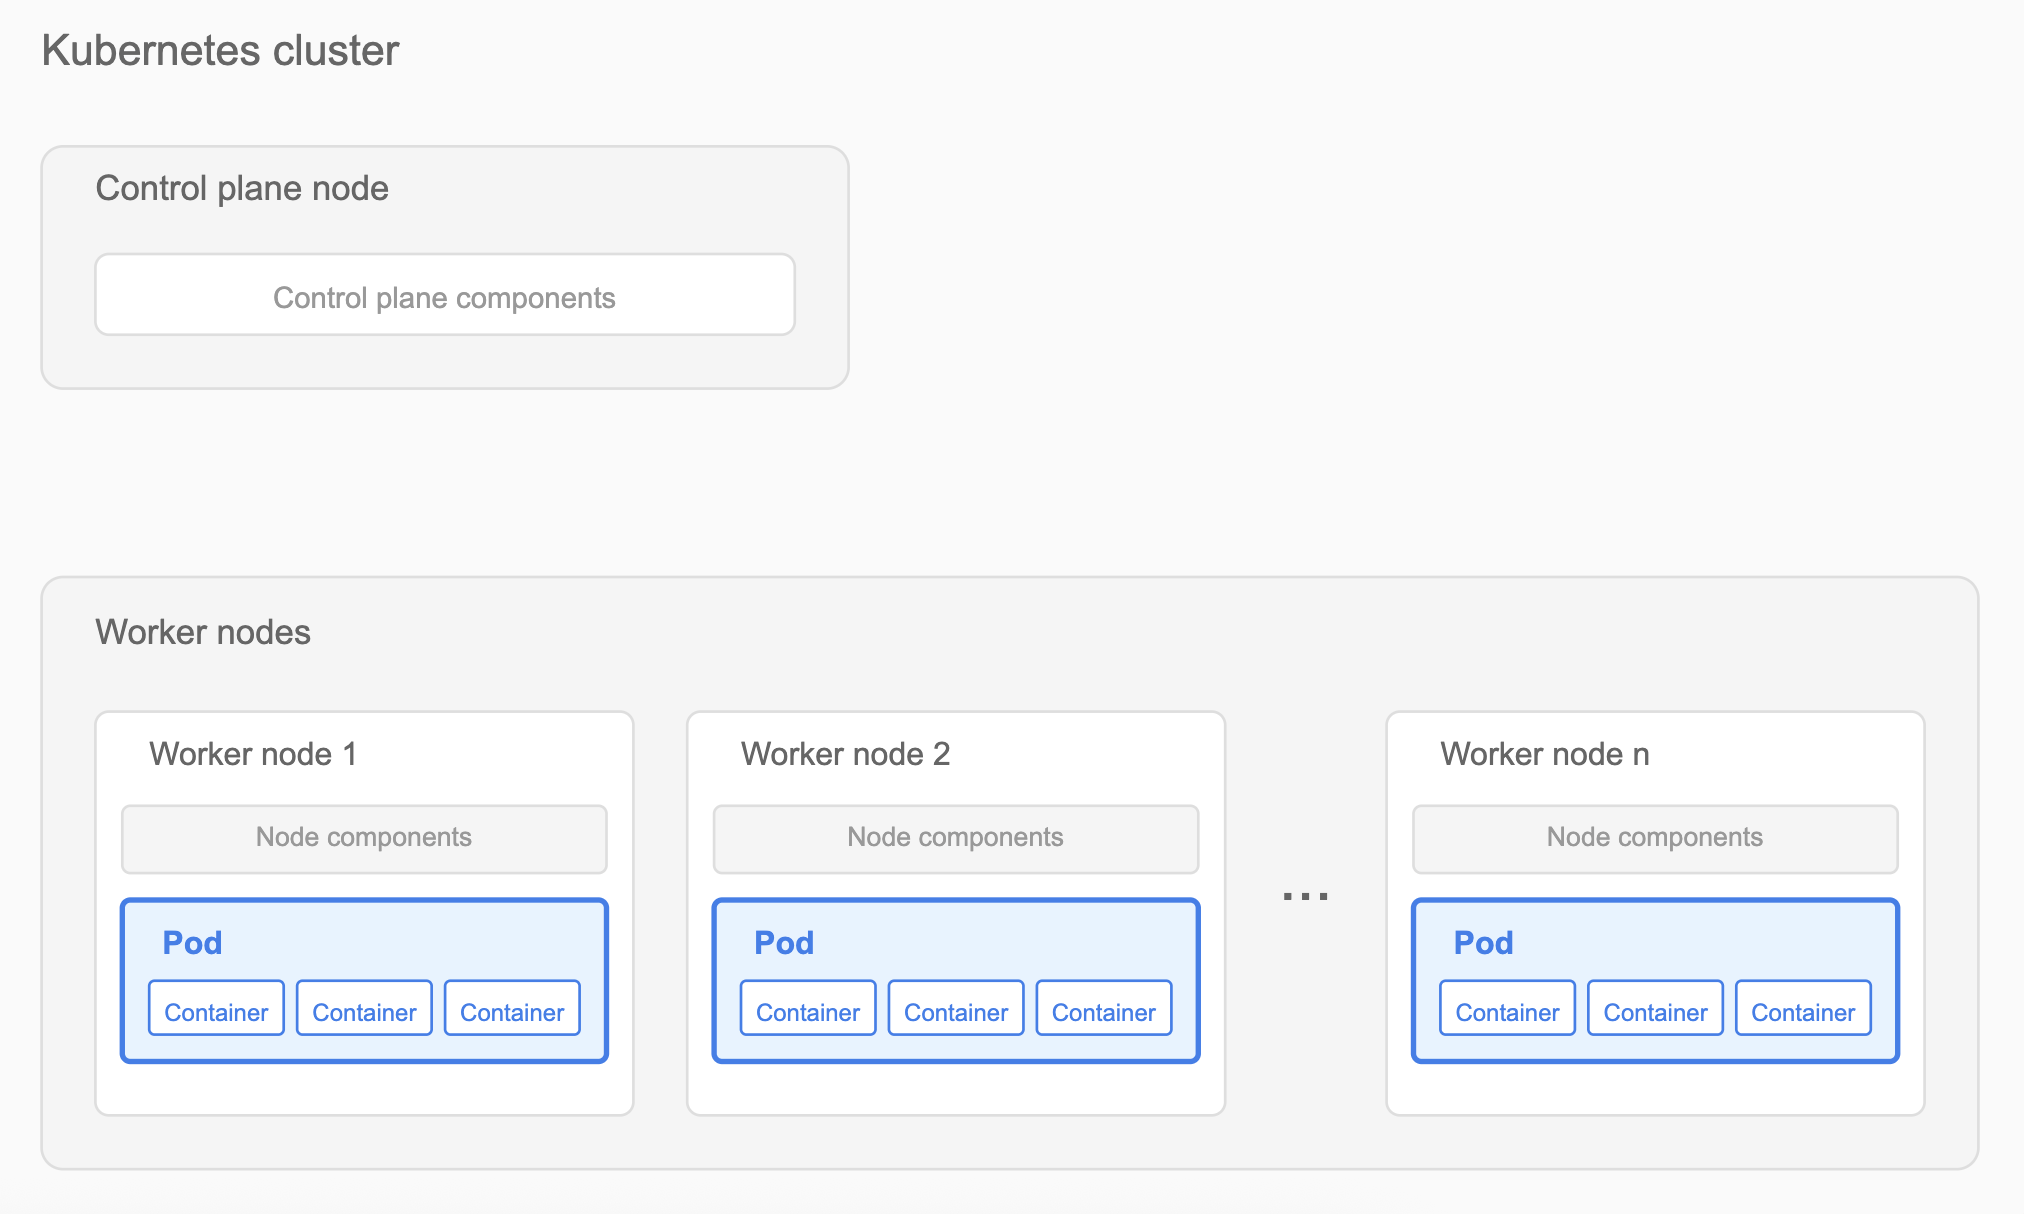
\includegraphics[width=0.6\textwidth]{images/cluster_architecture.png}
    \caption{Kubernetes cluster architecture}
    \label{fig:cluster}
\end{figure}

This article helps Kubernetes cluster administrators and developers diagnose and troubleshoot pod issues. After reading, you will be able to:

\begin{itemize}
    \item Inspect pod status in a cluster.
    \item Analyze logs for debugging.
    \item Execute shell commands within containers.
    \item Use ephemeral containers for interactive debugging.
\end{itemize}

\section*{Prerequisites}

Before starting, verify that you have:

\begin{itemize}
    \item Access to a Kubernetes cluster with running pods.
    \item Sufficient permissions to execute \texttt{kubectl} commands.
\end{itemize}

\section*{Debug pods in a Kubernetes cluster}

The following sections describe common debugging techniques. Use these techniques sequentially or combine them based on your specific scenario.

\subsection*{1. Check pod status}

Begin debugging by checking the status of your pods.

To list all pods:

\begin{lstlisting}[style=bash]
$ kubectl get pods
\end{lstlisting}

To list pods in a specific namespace:

\begin{lstlisting}[style=bash]
$ kubectl get pods --namespace=<namespace-name>
\end{lstlisting}

Example:

\begin{lstlisting}[style=bash]
$ kubectl get pods --namespace=default
\end{lstlisting}

Expected output:

\begin{lstlisting}[style=bash]
NAME                                    READY   STATUS             RESTARTS   AGE
hello-node-7b87cd5f68-2wp4m             1/1     Running            0          21m
nginx-deployment-66b6c48dd5-8k4h2       0/1     Pending            0          5m
redis-master-58db8984f-xp4c8            0/1     ImagePullBackOff   0          2m
\end{lstlisting}

\begin{tcolorbox}[colback=green!5!white,colframe=green!75!black,title=Tip]
If a pod is stuck in \texttt{Pending} status, check cluster resource availability running the following command:

\begin{lstlisting}[style=bash]
$ kubectl describe node <node-name>
\end{lstlisting}
\end{tcolorbox}

For a graphical interface, use the Kubernetes dashboard:

\begin{enumerate}
    \item Open the Kubernetes dashboard.
    \item Navigate to the \textit{Pods} section.
    \item Select a pod to view its details.
\end{enumerate}

\begin{figure}[H]
    \centering
    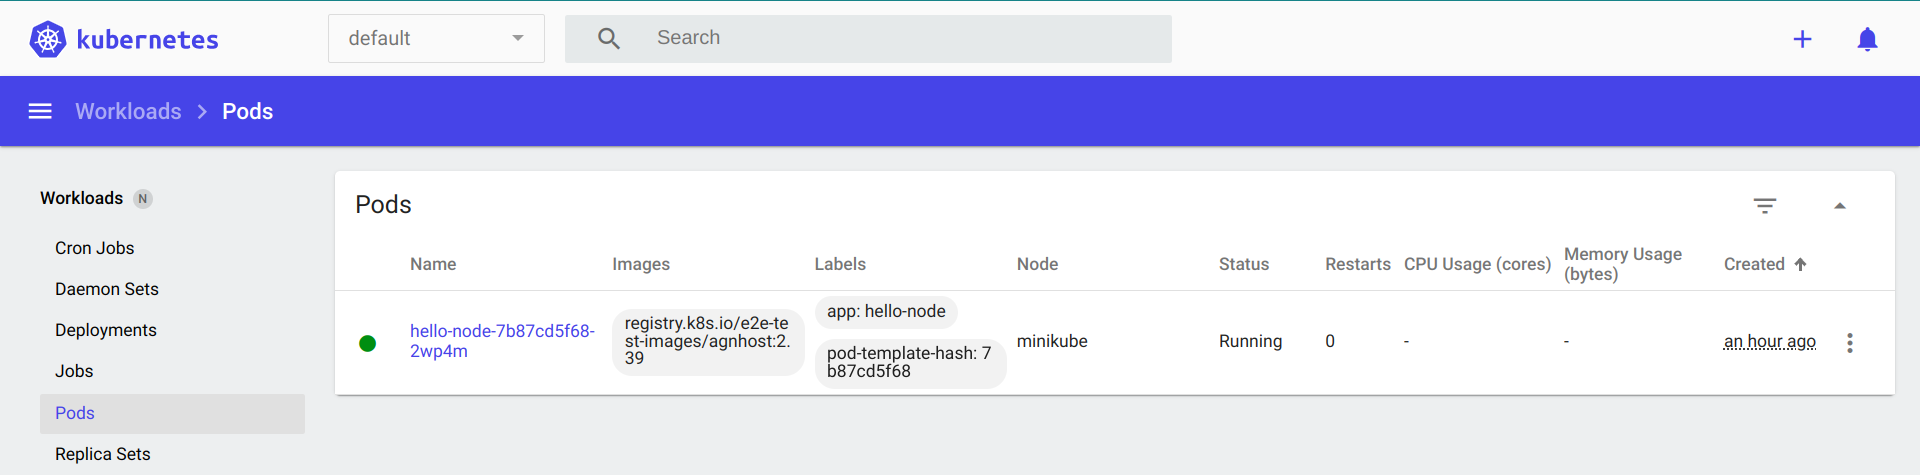
\includegraphics[width=0.7\textwidth]{images/pods.png}
    \caption{Pods in a Kubernetes dashboard}
    \label{fig:pods}
\end{figure}

\subsection*{2. Review pod logs}

Logs help identify what a container is doing or why it failed.

To view logs from all containers in a pod:

\begin{lstlisting}[style=bash]
$ kubectl logs <pod-name> --all-containers=true
\end{lstlisting}

To view logs from a specific container:

\begin{lstlisting}[style=bash]
$ kubectl logs <pod-name> -c <container-name>
\end{lstlisting}

\begin{tcolorbox}[colback=blue!5!white,colframe=blue!75!black,title=Note]
For pods with a single container, omit the container name.
\end{tcolorbox}

Example:

\begin{lstlisting}[style=bash]
$ kubectl logs hello-node-7b87cd5f68-2wp4m
\end{lstlisting}

Expected output:

\begin{lstlisting}[style=bash]
I0715 06:51:04.198447       1 log.go:195] Started HTTP server on port 8080
I0715 06:51:04.198572       1 log.go:195] Started UDP server on port 8081
\end{lstlisting}

\begin{tcolorbox}[colback=green!5!white,colframe=green!75!black,title=Tip]
For pods in \texttt{CrashLoopBackOff} status, check logs with the \texttt{--previous} flag to see the last container's logs before it crashed:

\begin{lstlisting}[style=bash]
$ kubectl logs <pod-name> --previous
\end{lstlisting}
\end{tcolorbox}

\subsection*{3. Execute container commands}

Inspect container state by running shell commands directly inside it.

Syntax:

\begin{lstlisting}[style=bash]
$ kubectl exec <pod-name> -c <container-name> -- <command>
\end{lstlisting}

\begin{tcolorbox}[colback=blue!5!white,colframe=blue!75!black,title=Note]
If not specified, commands run in the first container of the pod.
\end{tcolorbox}

Examples:

\textbf{Check container environment variables}

\begin{lstlisting}[style=bash]
$ kubectl exec nginx-deployment-66b6c48dd5-8k4h2 -- env
\end{lstlisting}

Expected output:

\begin{lstlisting}[style=bash]
PATH=/usr/local/sbin:/usr/local/bin:/usr/sbin:/usr/bin:/sbin:/bin
HOSTNAME=nginx-deployment-66b6c48dd5-8k4h2
NGINX_VERSION=1.21.1
NJS_VERSION=0.6.1
PKG_RELEASE=1~buster
HOME=/root
\end{lstlisting}

\textbf{Verify network connectivity}

\begin{lstlisting}[style=bash]
$ kubectl exec nginx-deployment-66b6c48dd5-8k4h2 -- curl -I localhost:80
\end{lstlisting}

Expected output:

\begin{lstlisting}[style=bash]
HTTP/1.1 200 OK
Server: nginx/1.21.1
Date: Tue, 14 Jan 2025 10:15:23 GMT
Content-Type: text/html
Content-Length: 612
Connection: keep-alive
\end{lstlisting}

\textbf{Check running processes}

\begin{lstlisting}[style=bash]
$ kubectl exec nginx-deployment-66b6c48dd5-8k4h2 -- ps aux
\end{lstlisting}

Expected output:

\begin{lstlisting}[style=bash]
USER       PID %CPU %MEM    VSZ   RSS TTY   STAT START   TIME COMMAND
root         1  0.0  0.1  10640  5548 ?     Ss   10:00   0:00 nginx: master process
nginx       31  0.0  0.1  11088  5164 ?     S    10:00   0:00 nginx: worker process
\end{lstlisting}

\begin{tcolorbox}[colback=green!5!white,colframe=green!75!black,title=Tip]
For containers that crash immediately, create a copy of the pod with a sleep command:

\begin{lstlisting}[style=bash]
$ kubectl debug <pod-name> --copy-to=<pod-name>-debug --container=<container-name> -- sleep 1d
\end{lstlisting}
\end{tcolorbox}

\subsection*{4. Use ephemeral debug containers}

Ephemeral containers let you attach debugging tools to running pods without modifying the original containers.

To create an ephemeral debug container:

\begin{lstlisting}[style=bash]
$ kubectl debug <pod-name> -it --image=<debug-image>
\end{lstlisting}

Examples:

\textbf{Debug networking issues using \texttt{netshoot}}

\begin{lstlisting}[style=bash]
$ kubectl debug nginx-deployment-66b6c48dd5-8k4h2 -it --image=nicolaka/netshoot
\end{lstlisting}

Expected output:

\begin{lstlisting}[style=bash]
Defaulting debug container name to debugger-nx8j2.
If you don't see a command prompt, try pressing enter.
~ # dig Kubernetes.default.svc.cluster.local
~ # curl -v telnet://nginx-service:80
~ # tcpdump -i any port 80
\end{lstlisting}

\textbf{Analyze memory usage with tools}

\begin{lstlisting}[style=bash]
$ kubectl debug redis-master-58db8984f-xp4c8 -it --image=ubuntu
\end{lstlisting}

Expected output:

\begin{lstlisting}[style=bash]
Defaulting debug container name to debugger-7xj4d.
If you don't see a command prompt, try pressing enter.
root@redis-master-58db8984f-xp4c8:/# apt-get update
root@redis-master-58db8984f-xp4c8:/# apt-get install -y procps
root@redis-master-58db8984f-xp4c8:/# top
...Memory usage details...
\end{lstlisting}

\begin{tcolorbox}[colback=green!5!white,colframe=green!75!black,title=Tip]
For pods with \texttt{ImagePullBackOff} status, verify image name and registry credentials. Check image pull secrets using:

\begin{lstlisting}[style=bash]
$ kubectl get pod <pod-name> -o=jsonpath='{.spec.imagePullSecrets[0].name}'
\end{lstlisting}
\end{tcolorbox}

\end{document}
